\section{Results}
\label{sec:results}

\subsection{How much signal is there?}
\label{sec:noise}

\begin{table}[t]
\centering
\caption{Signal against noise. Loss varies across mixtures over 100 times more than across seeds. Downstream accuracy varies across mixtures about as much as across seeds. In-domain loss covers runs that contain the domain.}
\label{tab:noise}
\begin{tabular}{@{}lcccc@{}}
\toprule
Metric & Range across mixtures & SD across mixtures & SD across seeds & Ratio \\
\midrule
In-domain loss (nats) & 0.7--1.5 & -- & 0.004--0.008 & $>100$ \\
$\Kzs$ (\%) & 26.0--28.7 & 0.39 & 0.26 & 1.5 \\
$\Kft$ (\%) & 39.0--49.1 & 1.35 & 0.55 & 2.4 \\
\listops (\%) & 35.5--42.2 & 1.03 & 0.76 & 1.3 \\
\proofwriter (\%) & 56.0--70.6 & 2.70 & 2.58 & 1.0 \\
$\Rc$ (\%) & 47.5--54.8 & 1.41 & 1.29 & 1.1 \\
Arithmetic (\%) & 7.7--98.5 & 25.6 & 23.4 & 1.1 \\
\bottomrule
\end{tabular}
\end{table}

\Tabref{tab:noise} sets the scale for everything that follows.
We measure loss two orders of magnitude more precisely than it varies.
Downstream accuracy is different: only the knowledge measures rise clearly above seed noise, and a few extreme mixtures drive that.
Pre-training does help the probes.
The randomly initialized control scores 37.6\% on $\Kft$, 30.1\% on \listops, and 55.9\% on \proofwriter, and the uniform mixture adds 9.3, 9.0, and 3.7 points.

\subsection{H1: in-domain loss is log-linear in the domain's share}
\label{sec:h1}

\begin{figure}[t]
\centering
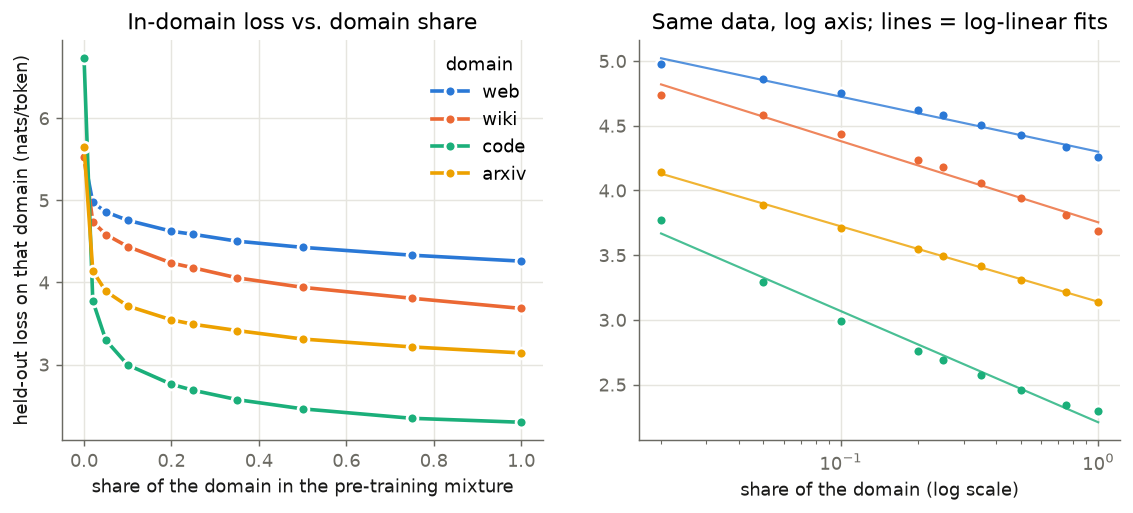
\includegraphics[width=0.95\linewidth]{figures/fig1_indomain_loss.png}
\caption{Held-out loss on each domain as its share of the mixture varies. \figleft Linear share axis. \figright The same points on a log axis with log-linear fits. Loss is close to a straight line in log share over the whole range from 2\% to 100\%, with no bend at 20\%.}
\label{fig:indomain}
\end{figure}

\begin{table}[t]
\centering
\caption{Curve-shape comparison for in-domain loss, fitted on the nine shares above zero. LOO is leave-one-out RMSE in nats per token; lower is better and the best is in {\bf bold}. ``Exp'' is the one-dimensional form of \citet{ye2025datamixing}.}
\label{tab:h1}
\resizebox{\textwidth}{!}{
\begin{tabular}{@{}lcccccccccc@{}}
\toprule
& \multicolumn{4}{c}{Loss at share} & \multicolumn{2}{c}{$R^2$} & \multicolumn{4}{c}{LOO error} \\
\cmidrule(lr){2-5} \cmidrule(lr){6-7} \cmidrule(lr){8-11}
Domain & 0 & 0.02 & 0.2 & 1.0 & Linear & Log & Linear & Log & Exp & Log+plateau \\
\midrule
\web & 5.53 & 4.97 & 4.62 & 4.26 & 0.863 & 0.984 & 0.120 & 0.044 & {\bf 0.041} & 0.051 \\
\wiki & 5.52 & 4.74 & 4.24 & 3.68 & 0.872 & 0.980 & 0.171 & 0.074 & {\bf 0.056} & 0.084 \\
\code & 6.73 & 3.77 & 2.76 & 2.30 & 0.669 & 0.984 & 0.369 & 0.095 & 0.163 & {\bf 0.074} \\
\arxiv & 5.65 & 4.14 & 3.55 & 3.14 & 0.769 & 0.9996 & 0.208 & {\bf 0.009} & 0.092 & 0.025 \\
\bottomrule
\end{tabular}}
\end{table}

\Figref{fig:indomain} and \tabref{tab:h1} show that H1 holds for loss.
The two-parameter log law beats the linear law in every domain, with 2.3 to 22 times lower LOO error, and it is the best or near-best model everywhere.
AICc agrees: the log law is 17--57 units below the linear law.

The law is a good approximation, not an exact description.
Residuals from the log law are 0.01--0.10 nats, which is still larger than seed noise (0.004--0.008) for \web, \wiki, and \code.
For \arxiv the fit is essentially exact.

\para{Share 0 is a cliff, not a point on the curve.}
The first 2\% of a domain delivers 43--67\% of the total improvement from 0\% to 100\%.
No smooth law fitted to $p > 0$ extrapolates to $p = 0$.

\subsection{H2: no saturation at 20\%}
\label{sec:h2}

\begin{table}[t]
\centering
\caption{Saturation analysis for in-domain loss. A plateau starting at 1.00 means the fit found no saturation inside the sweep.}
\label{tab:h2}
\begin{tabular}{@{}lcccccc@{}}
\toprule
& \multicolumn{3}{c}{\% of 0$\to$100\% gain reached at} & \multicolumn{2}{c}{Further gain 20\%$\to$100\%} & \\
\cmidrule(lr){2-4} \cmidrule(lr){5-6}
Domain & 5\% & 20\% & 50\% & nats & seed SDs & Fitted plateau start \\
\midrule
\web & 53 & 71 & 87 & 0.36 & 74 & 1.00 (none) \\
\wiki & 51 & 70 & 86 & 0.55 & 79 & 1.00 (none) \\
\code & 78 & 90 & 96 & 0.46 & 59 & 0.65 \\
\arxiv & 70 & 84 & 93 & 0.40 & 98 & 1.00 (none) \\
\bottomrule
\end{tabular}
\end{table}

Returns diminish in the sense that any logarithm does.
Each doubling of a domain's share buys a roughly constant 0.15 (\web), 0.20 (\wiki), 0.32 (\code), or 0.18 (\arxiv) nats.
But nothing special happens at 20\% (\tabref{tab:h2}).
Loss falls a further 0.36--0.55 nats between 20\% and 100\%, which is 59--98 seed standard deviations.
A log law with a plateau fits worse out of sample than a plain log law in three of four domains.
Where the data prefer a plateau, for \code, it starts at about 65\%.

\begin{figure}[t]
\centering
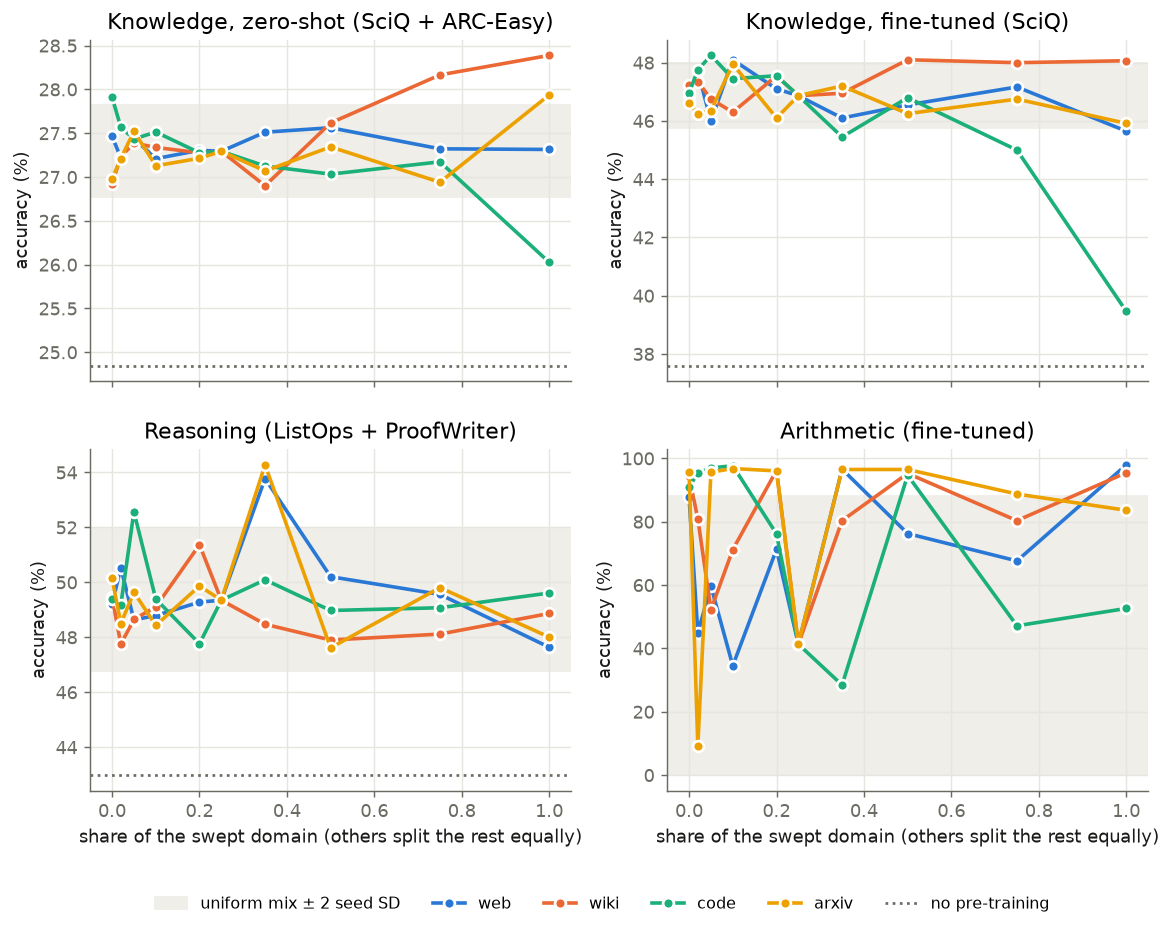
\includegraphics[width=0.95\linewidth]{figures/fig2_downstream_sweeps.png}
\caption{Downstream accuracy as each domain's share is swept. The grey band is the uniform-mixture mean $\pm 2$ pooled seed SD. Points are single seeds except at replicated shares, where they are means of three. Between shares of 2\% and 50\% every score stays inside the band.}
\label{fig:downstream}
\end{figure}

\para{Downstream tasks have no rising segment to saturate.}
Between shares of 2\% and 50\%, $\Kzs$, $\Kft$, and $\Rc$ stay inside the $\pm 2$ SD seed band for every domain (\figref{fig:downstream}).
The log law is also not the preferred shape for downstream scores.
A linear fit has the lowest LOO error in 8 of 12 downstream domain--metric pairs, because the only real effects sit at the high-share end: more \wiki raises knowledge scores and more \code lowers them.
This is the opposite of diminishing returns.
In most of these fits $R^2$ is below 0.25, so there is little to explain.

\subsection{H3: code is not a strong driver of reasoning scores}
\label{sec:h3}

\begin{figure}[t]
\centering
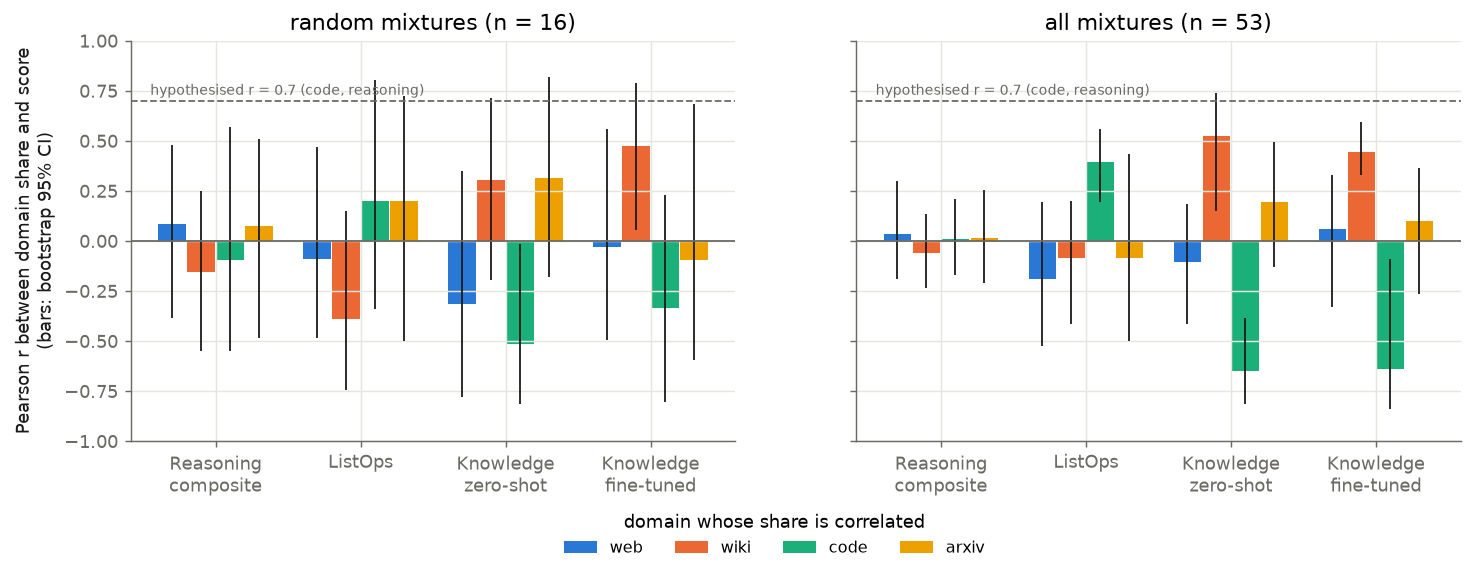
\includegraphics[width=0.95\linewidth]{figures/fig4_correlations.png}
\caption{Pearson correlation between each domain's share and downstream scores, on the 16 random mixtures (the pre-specified test) and on all 53 mixtures. No domain correlates with the reasoning composite; code share is the strongest negative correlate of both knowledge measures.}
\label{fig:corr}
\end{figure}

\begin{table}[t]
\centering
\caption{Correlation of code share with downstream scores, with bootstrap 95\% confidence intervals where computed. {\bf Bold} marks intervals that exclude zero. The last column names the domain with the strongest positive correlation on all mixtures.}
\label{tab:h3}
\begin{tabular}{@{}llll@{}}
\toprule
Score & Random mixtures ($n=16$) & All mixtures ($n=53$) & Strongest domain \\
\midrule
$\Rc$ & $-0.10$ $[-0.55, 0.57]$ & $0.01$ $[-0.17, 0.21]$ & none (all $|r| < 0.07$) \\
\listops & $0.20$ $[-0.34, 0.81]$ & ${\bf 0.39}$ $[0.19, 0.56]$ & \code \\
\proofwriter & $-0.20$ & $-0.14$ & none significant \\
$\Kzs$ & $-0.52$ & ${\bf -0.65}$ $[-0.82, -0.39]$ & \wiki ($+0.52$) \\
$\Kft$ & $-0.34$ & ${\bf -0.64}$ $[-0.84, -0.09]$ & \wiki ($+0.45$) \\
\bottomrule
\end{tabular}
\end{table}

The hypothesized $r > 0.7$ is far from what we observe (\figref{fig:corr}, \tabref{tab:h3}).
On the random mixtures, code share correlates with $\Rc$ at $r = -0.10$, and even the upper confidence limit of 0.57 is below 0.7.
On all 53 mixtures $r = 0.01$.
Removing code entirely changes nothing we can measure: $\Rc$ is 49.4\% without code and 49.4\% at uniform.

\para{Does code help any reasoning task?}
Code has the largest positive association with one task, \listops, which is the most code-like of our probes because its inputs are bracketed nested operators ($r = 0.39$, Holm-corrected $p = 0.014$).
The effect is small.
A mixture regression predicts 41.4\% (SE 0.6) for a pure-code corpus against 38.6--39.3\% for the other pure corpora, and the seed-replicated pure-code model is 1.6 points above uniform (Welch $p = 0.14$, 3 vs.\ 3 seeds).

\subsection{H4: web text above 50\% does not measurably hurt knowledge tasks}
\label{sec:h4}

\begin{figure}[t]
\centering
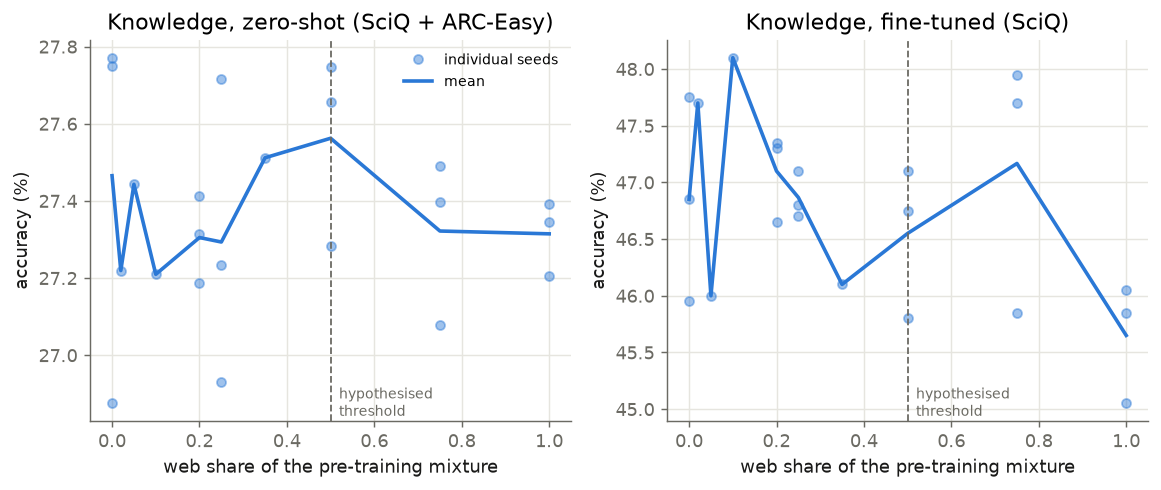
\includegraphics[width=0.8\linewidth]{figures/fig3_web_knowledge.png}
\caption{Knowledge accuracy along the web sweep. Dots are individual seeds. Neither measure drops between 50\% and 75\% web; only the pure-web model is lower, and only on $\Kft$.}
\label{fig:web}
\end{figure}

\begin{table}[t]
\centering
\caption{Web sweep with three seeds per point (mean $\pm$ SD across seeds). Loss on the knowledge-bearing domains rises smoothly past 50\% web and collapses at 100\%; the accuracy measures do not track it.}
\label{tab:h4}
\begin{tabular}{@{}lcccc@{}}
\toprule
Web share & $\Kzs$ (\%) & $\Kft$ (\%) & \wiki loss & \arxiv loss \\
\midrule
0 & 27.47 {\scriptsize $\pm$ 0.51} & 46.85 {\scriptsize $\pm$ 0.90} & 4.18 & 3.43 \\
0.25 (uniform) & 27.29 {\scriptsize $\pm$ 0.40} & 46.87 {\scriptsize $\pm$ 0.21} & 4.18 & 3.49 \\
0.50 & 27.56 {\scriptsize $\pm$ 0.25} & 46.55 {\scriptsize $\pm$ 0.67} & 4.20 & 3.58 \\
0.75 & 27.32 {\scriptsize $\pm$ 0.22} & 47.17 {\scriptsize $\pm$ 1.15} & 4.28 & 3.76 \\
1.00 & 27.31 {\scriptsize $\pm$ 0.10} & 45.65 {\scriptsize $\pm$ 0.53} & 5.29 & 6.09 \\
\bottomrule
\end{tabular}
\end{table}

At 75\% web, both knowledge measures are statistically indistinguishable from 50\% or 25\% (all $p > 0.27$; \figref{fig:web}, \tabref{tab:h4}).
The pure-web model is 1.2 points below uniform on $\Kft$ (Welch $t = -3.7$, $p = 0.043$, uncorrected, 3 vs.\ 3 seeds) and unchanged on $\Kzs$.
We do not read much into this single result.
We examined about ninety such contrasts, so it would not survive a multiplicity correction, and ``all web'' is also ``no Wikipedia and no papers at all''.

Loss does respond to web share.
Loss on \wiki rises from 4.20 to 4.28 and loss on \arxiv from 3.58 to 3.76 as web grows from 50\% to 75\%, and both collapse at 100\%.
The accuracy measures do not follow.

\para{What does hurt knowledge scores?}
Code at very high shares.
Pure code is 7.4 points below uniform on $\Kft$ (39.5\% vs.\ 46.9\%, $t = -28$) and 1.3 points below on $\Kzs$; 75\% code is about 1.9 points below on $\Kft$ (single seed).
Pure Wikipedia is the best knowledge model, 1.2 points above uniform on $\Kft$ and 1.1 on $\Kzs$ ($p = 0.05$ and $0.02$, uncorrected).

\subsection{Can a mixture law predict unseen mixtures?}
\label{sec:laws}

\begin{figure}[t]
\centering
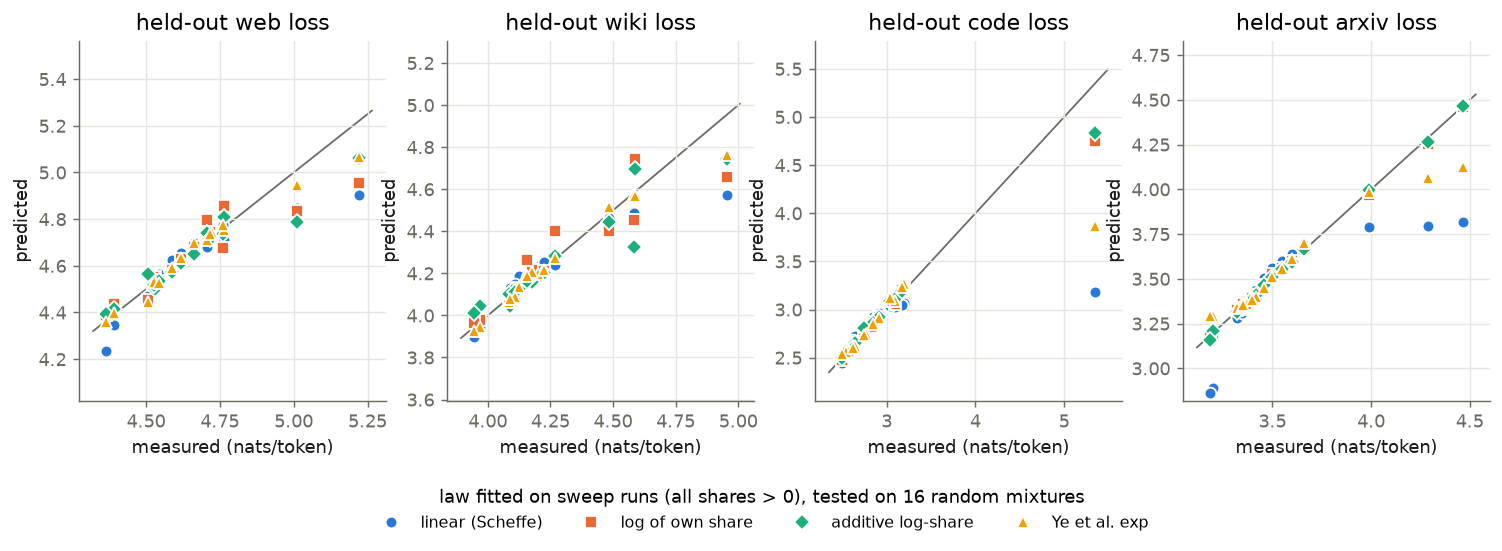
\includegraphics[width=0.95\linewidth]{figures/fig5_law_prediction.png}
\caption{Predicted against observed scores on the 16 held-out random mixtures, for laws fitted on the 29 structured mixtures with every share above zero. Loss is predictable; downstream scores are not predictable beyond noise.}
\label{fig:laws}
\end{figure}

\begin{table}[t]
\centering
\caption{Test RMSE (nats per token) of mixture laws on 16 held-out random mixtures. Parameter counts are in parentheses. Best per row in {\bf bold}.}
\label{tab:laws}
\resizebox{\textwidth}{!}{
\begin{tabular}{@{}lccccc@{}}
\toprule
Held-out loss & Predict the mean & Linear (4) & Log of own share (2) & Additive log-share (5) & Exponential (6) \\
\midrule
\web & 0.215 & 0.100 & 0.092 & 0.073 & {\bf 0.047} \\
\wiki & 0.262 & 0.110 & 0.102 & 0.094 & {\bf 0.051} \\
\code & 0.681 & 0.547 & 0.153 & {\bf 0.132} & 0.372 \\
\arxiv & 0.360 & 0.238 & 0.014 & {\bf 0.011} & 0.109 \\
\bottomrule
\end{tabular}}
\end{table}

\para{Loss is predictable.}
A log-share law predicts loss on unseen mixtures with correlation 0.94--0.9996 (\figref{fig:laws}, \tabref{tab:laws}).
No single form wins.
The exponential law of \citet{ye2025datamixing} is best where domains help each other (\web and \wiki), and log-share laws extrapolate far better to tiny shares; the random set includes shares as small as 0.1\%.
The errors of all laws concentrate on the three random mixtures with a share below the fitted range of 2\% (0.1\% code, 0.6\% and 1.2\% arXiv).

\begin{table}[t]
\centering
\caption{Transfer matrix of the additive log-share law (\eqref{eq:additive}): change in loss on the row domain, in nats, per $e$-fold increase in the share of the column domain. Bootstrap SE is at most 0.04. Own-domain effects are in {\bf bold}.}
\label{tab:transfer}
\begin{tabular}{@{}lcccc@{}}
\toprule
Loss on $\downarrow$ / share of $\rightarrow$ & \web & \wiki & \code & \arxiv \\
\midrule
\web & ${\bf -0.22}$ & $-0.08$ & $0.00$ & $0.01$ \\
\wiki & $-0.08$ & ${\bf -0.29}$ & $0.01$ & $0.01$ \\
\code & $-0.05$ & $-0.04$ & ${\bf -0.46}$ & $-0.03$ \\
\arxiv & $-0.01$ & $-0.01$ & $0.00$ & ${\bf -0.26}$ \\
\bottomrule
\end{tabular}
\end{table}

\para{Which domains help each other?}
The additive law gives an interpretable transfer matrix (\tabref{tab:transfer}).
Web and Wikipedia help each other at roughly a third of the own-domain rate.
Loss on arXiv and on code depends almost only on the domain's own share.

\para{Downstream scores are not predictable from the mixture beyond noise.}
On the held-out random mixtures the linear mixture model reaches $r = 0.52$ for $\Kft$ and $0.56$ for \listops, but only $0.20$ for $\Kzs$ and $0.18$ for $\Rc$, with RMSE equal to or worse than predicting the mean for $\Kzs$ and $\Rc$.

\para{Is loss a proxy for downstream scores?}
Only weakly.
Across mixtures, $\Kft$ tracks mean natural-language loss with Spearman $\rho = -0.59$ and $\Kzs$ with $\rho = -0.44$.
The reasoning scores track no loss ($|\rho| \le 0.39$, and $\le 0.15$ for the composite).
